\documentclass[xcolor=x11names,compress]{beamer}
\usepackage[utf8]{inputenc}

%% packages
\usepackage{graphicx}
\usepackage{hyperref}
\usepackage{amsmath}
\usepackage{amssymb}

%% hyperlinks
\hypersetup{
	colorlinks=true,
	linkcolor=blue,
	filecolor=blue,      
	urlcolor=blue,
	citecolor=blue
}

%% self-commands
\newcommand{\As}{\textit{Anabaena sp.}}
\newcommand{\Ss}{\textit{Synechocystic sp.}}
\newcommand{\Cs}{\textit{Chroococcidiopsis sp.}}
\newcommand{\Ct}{\textit{Chroococcidiopsis thermalis}}

\title{MRes: Eco-bioelectric Cell}
\author{PokMan Ho}
\date{16 January 2020}

\begin{document}

\begin{frame}
    \maketitle
\end{frame}

\begin{frame}{Computer Model Visualization}
    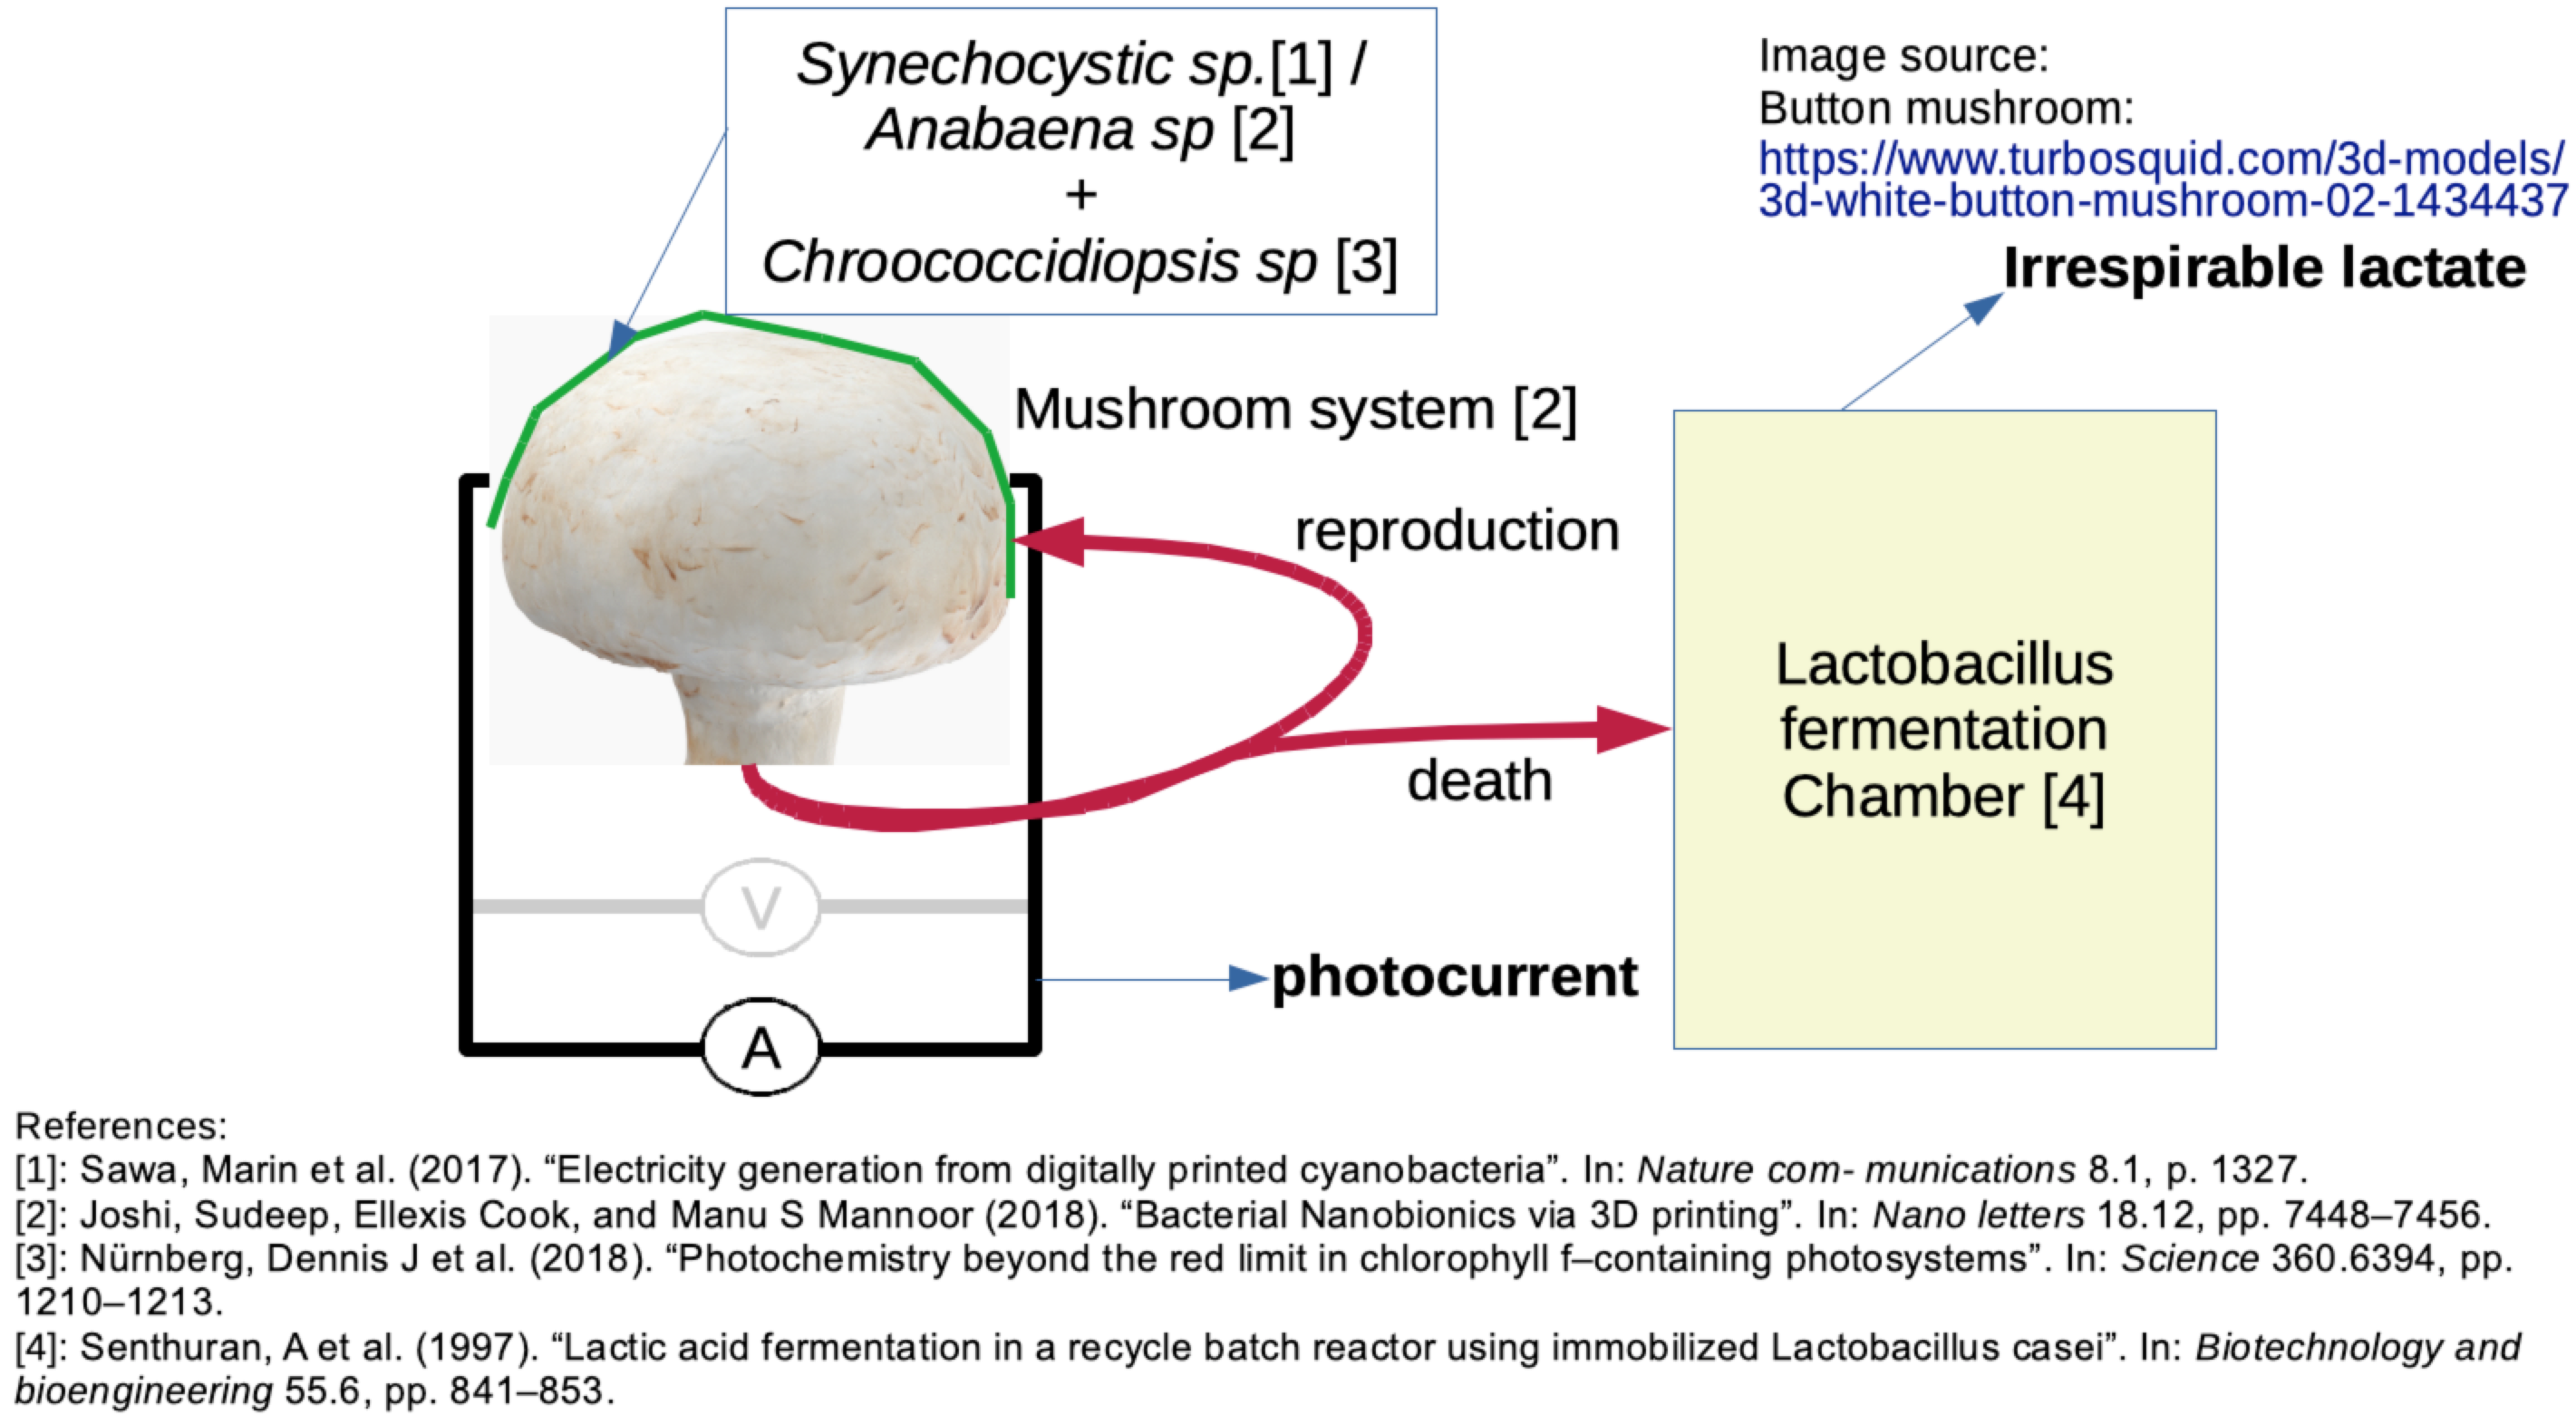
\includegraphics[width=\linewidth]{figure/proposed_model.png}
\end{frame}

\begin{frame}{Computer Model in Equations}
    pillar equation:
    \begin{equation}\label{eq:main}
        dp/dt = r_p [p] - k_{p1} [p][q]
    \end{equation}
    population growth rate:
    \begin{equation}\label{eq:growth}
        r_p = \dfrac{r_p|_{expt}}{P_p|_{expt}}\cdot P_p = \dfrac{r_p|_{expt}\cdot t_p|_{expt}}{J_p|_{expt}}\cdot\dfrac{J_p}{3600}
    \end{equation}
    competition coefficient:
    \begin{equation}\label{eq:compete}
        k_{p1} = \dfrac{P_q}{P_p + P_q}\cdot r_p = \dfrac{J_q J_p}{(J_p + J_q)\cdot3600}\cdot \dfrac{r_p|_{expt}\cdot t_p|_{expt}}{J_p|_{expt}}
    \end{equation}
    Overall equation (will be used in script):
    \begin{tabular}{rll}
        $\dfrac{dp}{dt}$ & = $[p]\cdot(r_p - k_{p1}[q]) = [p]\cdot r_p(1-\dfrac{P_q}{P_p + P_q})$\\
         & = $[p]\cdot(\dfrac{r_p|_{expt}\cdot t_p|_{expt}}{J_p|_{expt}})\cdot\dfrac{J_p}{3600}\cdot\dfrac{J_p}{J_p + J_q}$
    \end{tabular}
\end{frame}

\end{document}
